% SVM parameter
\newcommand{\svmT}{\bm{\theta}}
\newcommand{\svmB}{b}
\newcommand{\svmAug}{\tilde{\svmT}}
%\newcommand{\svmAugAll}{\svmAug_{\text{all}}}
\newcommand{\svmAugAll}{\bm{\Theta}}

\begin{figure}
\begin{center}
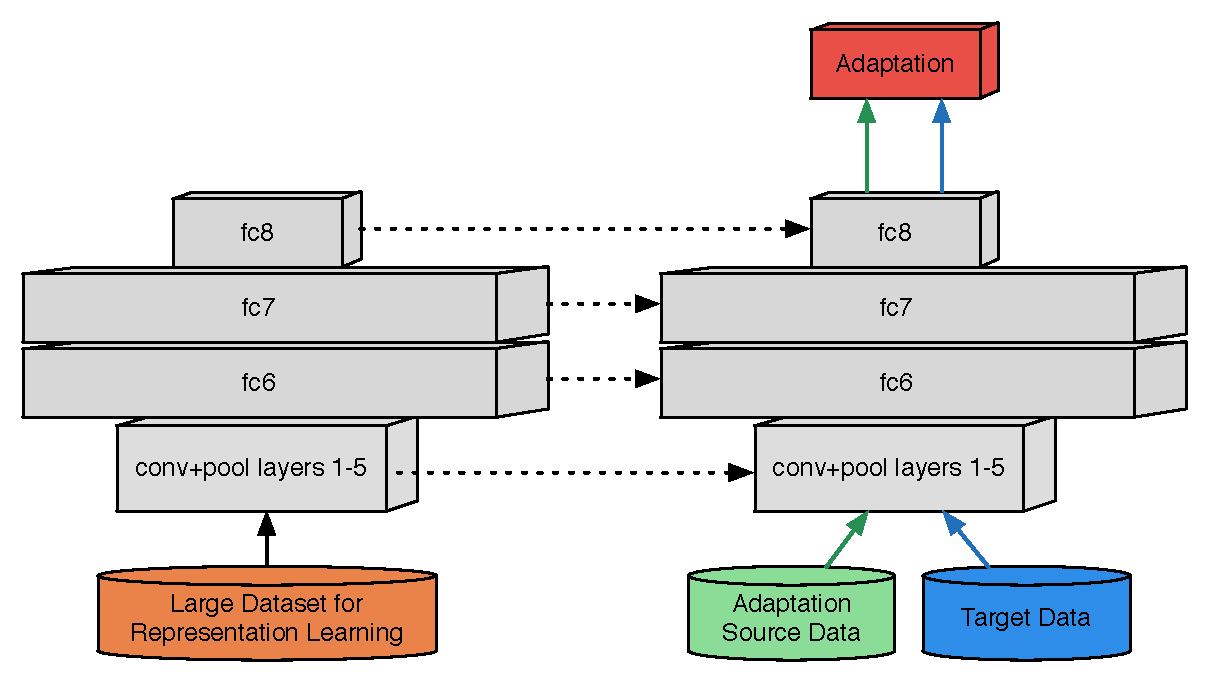
\includegraphics[width=.7\linewidth]{figs/model-adapt}
\end{center}
\caption{Our proposed framework for adaptation. The source data and target data are each independently passed through the supervised convolutional neural network which has been trained on the 1.2Million images in the ILSVRC2012 Challenge dataset~\cite{ilsvrc2012}. We compute the subspace distance (A-distance) between the source and target data as it is represented in each of the fully connected layers of the network (represented in blue). The layer that produces the minimum subspace distance between source and target is chosen for adaptation. Finally, adaptation is performed on the activations from the best layer (shown in red).}
\label{fig:model}
\end{figure}

% Describe adaptation algorithms
%Many methods have been proposed for visual domain adaptation. 
% \ks{similar edit as in intro, see if this make sense}

We propose a general framework for selectively adapting the parameters of a
convolutional neural network (CNN) whose representation and classifier weights
are trained on a large-scale source domain, such as ImageNet. First, we make use
of the A-distance metric \et{(citation needed)} to automatically select a layer
from the CNN that will allow for effective adaptation. Next, our framework adds
a final domain-adaptive classification ``layer'' that takes the activations of
one of the existing network's layers as input features. This adapted layer is a
linear classifier that combines source and target training data using an
adaptation method. To demonstrate the generality of our framework, we select a
representative set of popular linear classifier adaptation approaches that we
empirically evaluate in Section~\ref{sec:eval}.

\subsection{Selecting a Layer for Adaptation}

Intuitively, when selecting a layer to use for adaptation, we would like to use
the one in which the source and target appear the most similar (and thus
experience the least domain shift).

To get at this notion of similarity, we make use of the concept of an A-distance
\et{citation needed}. The A-distance is a measure of how distinguishable
two datasets are. We compute a close approximation to the A-distance between
each of the domain shifts by training classifiers to identify which domain each
image comes from. The A-distance between two domains $X_1$ and $X_2$ is then
simply given by

\begin{equation}
  d_A(X_1, X_2) = 2 \left( 1 - 2E(X_1, X_2)\right)
\end{equation}


where $E(X_1, X_2)$ is the test error of the classifier attempting to
distinguish between the two domains.

After computing A-distances between domain shifts for each of the
fully-connected layers in the CNN, we simply select the layer that produces the
smallest A-distance for use at adaptation time.

\subsection{Applying Adaptation Techniques}

Once we have selected which layer to use, we then add an adaptation ``layer'' to
the top of the architecture, as indicated in Figure~\ref{fig:model}. This layer
consists of an adaptation technique which combines the source and target
training data, then learns a linear classifier. In this paper, we look to the
standard domain adaptation literature and experiment using a variety of those
techniques.

We are interested in both unsupervised and supervised settings, so we examine
two sets of adaptation techniques. For the unsupervised setting, we use the
Geodesic Flow Kernel (GFK)~\cite{gong-cvpr12} and Subspace Alignment
(SA)~\cite{sa} methods. For the supervised setting, we use the Late Fusion,
\daume~\cite{daume}, Projective Model Transfer (PMT)~\cite{aytar-iccv11}, and
Max-margin Domain Transforms (MMDT)~\cite{hoffman-iclr13} methods.
